\documentclass[14pt]{article}

\usepackage[utf8x]{inputenc}
\usepackage[russian]{babel}
\usepackage{graphicx}
\graphicspath{{images/}}
\DeclareGraphicsExtensions{.pdf,.png,.jpg}

\usepackage{amsmath}

\usepackage{geometry} % Меняем поля страницы
\geometry{left=2cm}% левое поле
\geometry{right=1.5cm}% правое поле
\geometry{top=2cm}% верхнее поле
\geometry{bottom=2cm}% нижнее поле

\renewcommand{\theenumi}{\arabic{enumi}}% Меняем везде перечисления на цифра.цифра
\renewcommand{\labelenumi}{\arabic{enumi}}% Меняем везде перечисления на цифра.цифра
\renewcommand{\theenumii}{.\arabic{enumii}}% Меняем везде перечисления на цифра.цифра
\renewcommand{\labelenumii}{\arabic{enumi}.\arabic{enumii}.}% Меняем везде перечисления на цифра.цифра
\renewcommand{\theenumiii}{.\arabic{enumiii}}% Меняем везде перечисления на цифра.цифра
\renewcommand{\labelenumiii}{\arabic{enumi}.\arabic{enumii}.\arabic{enumiii}.}% Меняем везде перечисления на цифра.цифра

\begin{document}

	\begin{titlepage}
	\begin{center}
		\fontsize{18pt}{20pt}\selectfont
		\textbf{Работа 1.1.1.}	
	
		\vspace{5cm}
		\fontsize{24pt}{25pt}\selectfont
		Определение систематических и случайных погрешностей при измерении удельного сопротивления нихромовой
		проволоки
	\end{center}
	\begin{flushright}
		\fontsize{18pt}{20pt}\selectfont
		\vspace{13cm}
		\hspace{-3cm}
		\textit{Корнеев Е.С.}
	
		\textit{Алферова А.В.}
	\end{flushright}		
	
	\end{titlepage}


	\begin{center}
	\fontsize{16pt}{18pt}\selectfont	
	Определение систематических и случайных погрешностей при измерении удельного сопротивления нихромовой
	проволоки
	\end{center}
	
	\fontsize{14pt}{16pt}\selectfont
	\vspace{1cm}
	\textbf{Цель работы:} измерить удельное сопротивление проволоки и вычислить систематические и случайные 									погрешности при использовании таких приборов, как линейка, штангенциркуль, микрометр, амперметр, вольтметр и мост 						постоянного тока.
	
	\vspace{0.5cm}
	\textbf{В работе используются:} линейка, штангенциркуль, микрометр, отрезок проволоки из нихрома, амперметр, вольтметр, 	источник 		ЭДС, мост постоянного тока, реостат, ключ.
	
	\vspace{1cm}
	\textbf{Ход работы:}
	\vspace{0.5cm}
	
	1. Определим точность приборов: \\
	\hspace*{2cm}штангенциркуль - 0.1 мм,\\
	\hspace*{2cm}микрометр - 0.01 мм
	
	\vspace{0.5cm}
	2. Измерим диаметр проволоки в нескольких местах штангенциркулем (\(d_1\)) и микрометром (\(d_2\)):\\
	\begin{center}
	\begin{tabular}{|l|c|c|c|c|c|c|c|c|c|c|}
	\hline
					& 1		& 2 	& 3		& 4 	& 5		& 6 	& 7		& 8		& 9		& 10\\
	\hline
	\(d_1\), мм 	& 0.4	& 0.4	& 0.4	& 0.4	& 0.4	& 0.4	& 0.4	& 0.4	& 0.4	& 0.4\\
	\hline
	\(d_2\), мм 	& 0.37	& 0.36	& 0.36	& 0.35	& 0.36	& 0.36	& 0.37	& 0.35	& 0.36	& 0.36\\
	\hline
	\multicolumn{11}{|c|}{$\langle d_1 \rangle = 0.4$мм \hspace{1cm}$\langle d_2 \rangle = 0.360$мм}\\	
	\hline
	\end{tabular}
	\end{center}
	

	\vspace{0.5cm}
	При измерении \(d_1\) штангенциркулем случайная погрешность отсутствует, следовательно, точность результата определяется только 		точностью штангенциркуля (систематическая погрешность):
	
	$$d_1 = (0.4 \pm 0.1)~\text{мм}$$ 
	
	Измерения микрометром содержат как ситематическую, так и случайную погрешности:
	
	$$\sigma_\text{сист} = 0.01~\text{мм}$$	
	
	$$\sigma_\text{сл} = \frac{1}{2}\sqrt{\sum_{i=1}^{N}(d_i - \langle d\rangle)^2\mathstrut}~=~\frac{1}{2}\sqrt{4*10^{-4}}					~=~2*10^{-3}~\text{мм}$$
	
	$$\sigma = \sqrt{\sigma_\text{сист}^2 + \sigma_\text{сл}^2\mathstrut}~=~\sqrt{(0.01)^2 + (0.002)^2\mathstrut}~\approx~0.01~				\text{мм}$$
	
	Так как $\sigma_\text{сл}^2 \flqq \sigma_\text{сист}^2$, то можно считать проволоку однородной, а погрешность диаметра 					$\sigma_d = \sigma_text{сист}$:
	
	$$d_2~=~\langle d_2\rangle \pm \sigma_d~=~(3.60 \pm 0.10)*10^{-2}~\text{см}$$
	
	\vspace{0.5cm}
	3. Определим площадь поперечного сечения проволоки $S$:
	
	$$S = \frac{\pi *(d_2)^2}{4} = \frac{3.14 * (3.60 * 10^{-2})^2}{4} = 1.02*10^{-3}~\text{см}$$
	
	Погрешность $\sigma_s$ найдем по формуле:
	
	$$\sigma_s = 2\frac{\sigma_d}{d}*S = 2*\frac{0.01}{0.36}*1.02*10^{-3} \approx 6*10^{-5}~\text{см}^2$$
	
	Таким образом, $S = (1.02 \pm 0.06)*10^{-3}~\text{см}^2$, то есть $S$ определена с точностью 6\%.
	
	\vspace{0.5cm}
	4. Определим основные характеристики приборов:
	
	\begin{center}
	\begin{tabular}{|p{0.35\linewidth}|p{0.25\linewidth}|p{0.25\linewidth}|}
	\hline
								& Вольтметр 		& Миллиамперметр\\
	\hline
	Предел измерений $x_n$ 		& 					& 0.75 A\\
	\hline
	Число делений $n$			& 					& 150 дел\\
	\hline
	Цена делений $x_n/n$		&					& 5 мА/дел\\
	\hline
	Чувствительность $n/x_n$	&					& 200 дел/мА\\
	\hline
	Внутреннее сопротивление	& 200 МОм			& ~\\	
	\hline	
	\end{tabular}
	\end{center}

	\vspace{1cm}
	5. Для нахождения значения сопротивления проволоки мы можем воспользоваться двумя схемами (рис. 1), где:
	
	\vspace*{0.3cm}
	$R_A$ - внутренее сопротивление амперметра;
	
	$R_V$ - внутреннее сопротивление вольтметра;
	
	$R_n$ - сопротивление куска нихромовой проволоки;
	
	$R$ - реостат.

	\newpage
	\vspace*{2cm}
	\begin{figure}[h!]
		\center{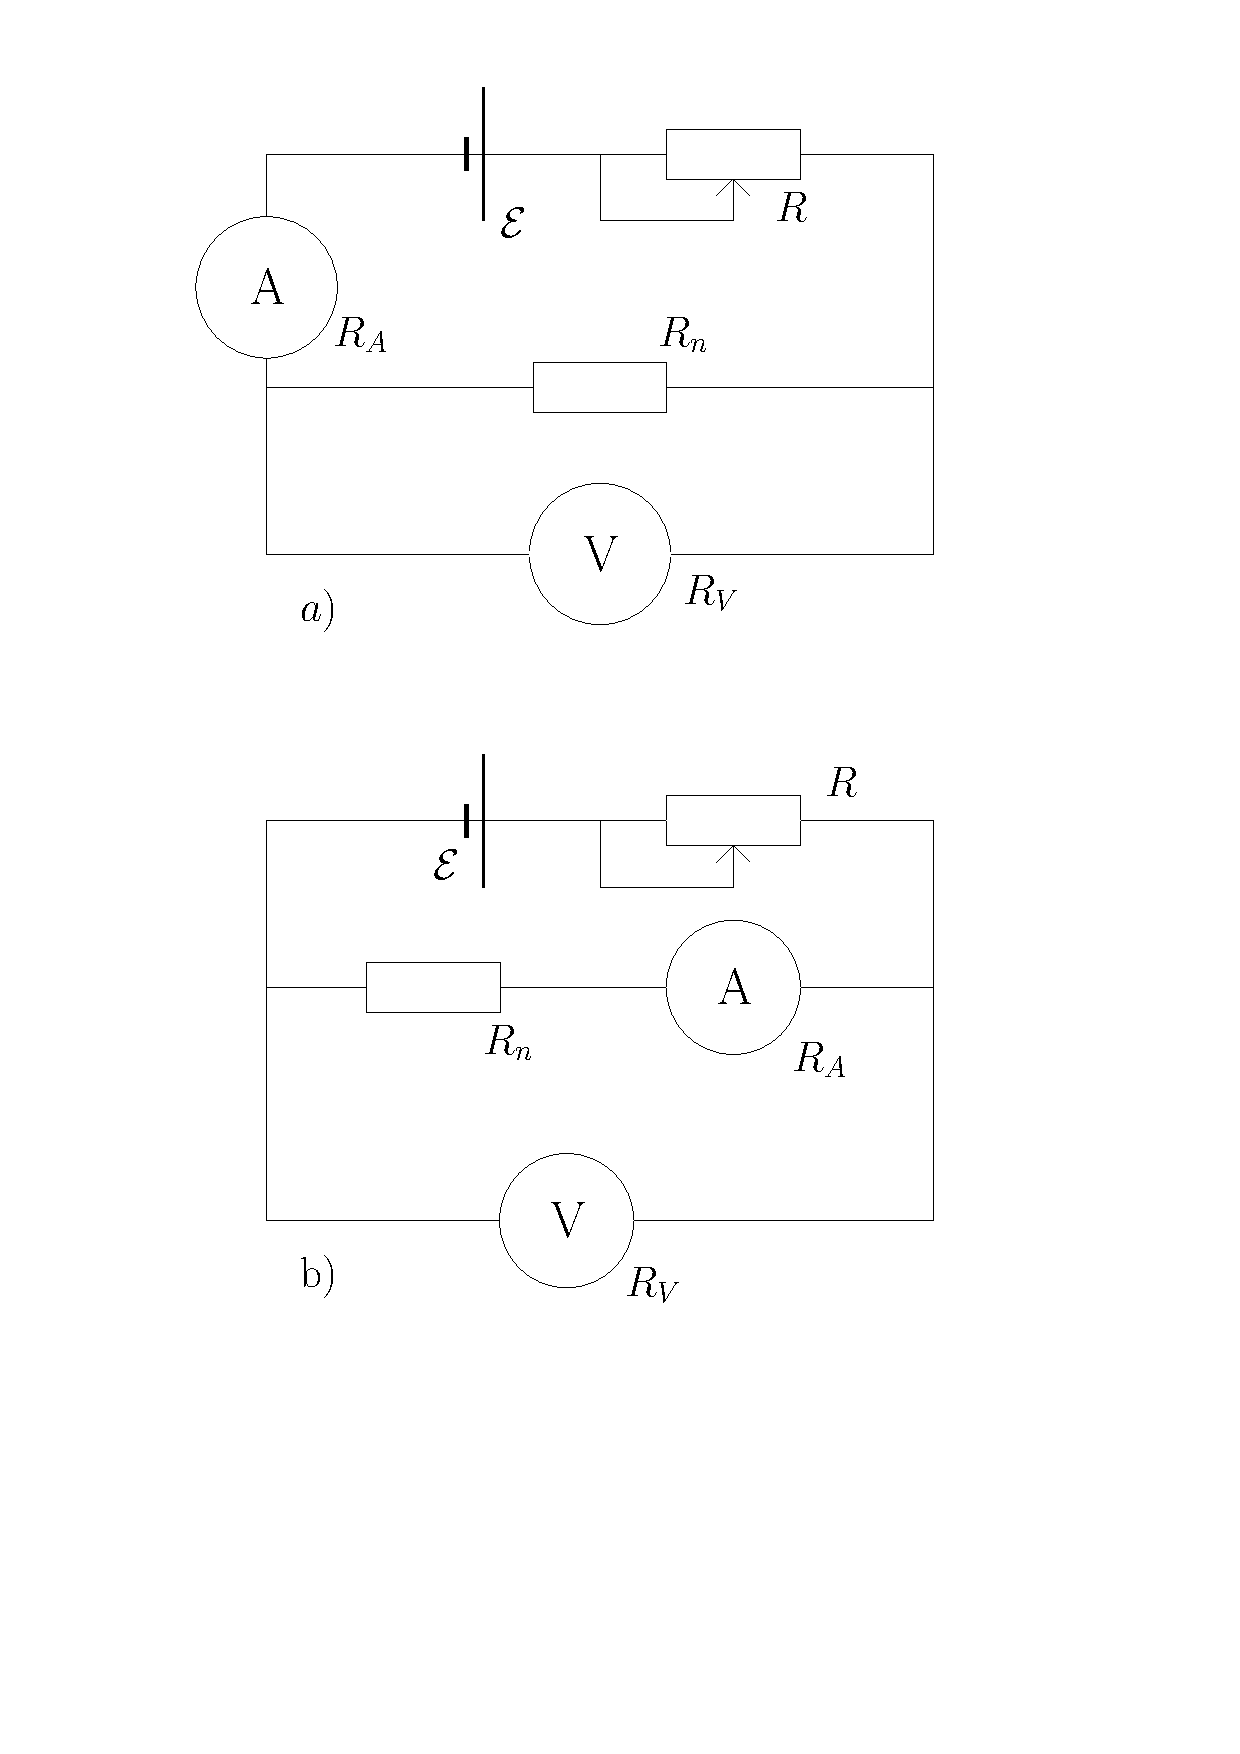
\includegraphics[width = 10cm]{scheme.pdf}}
		\caption{Схемы установок}
		\label{fig:image}
	\end{figure}
	
	\newpage
	
	Если обозначить показания вольтметра и амперметра через $V$ и $I$, то значения $R_{n1} = \frac{V_a}{I_a}$ и $R_{n2} = \frac{V_b}		{I_b}$ будут отличаться от реального $R_n$:
	
	$$R_{n1} = \frac{V_a}{I_a} = R_n\frac{R_V}{R_V + R_n} \Rightarrow R_n \approx R_{n1}\left( 1 + \frac{R_{n1}}{R_V} \right)$$
	
	$$R_{n2} = \frac{V_b}{I_b} = R_n + R_A \Rightarrow R_n \approx R_{n2} \left(1 - \frac{R_A}{R_{n2}}\right)$$

	Зная, что $R_n \approx 5$ Ом, оценим величину поправок:

%%%%%%%%%%%%%%%%%%%%%%%%%%%%%%%%%%%%%%%%%%%%%%%%%%%%%%%%%%%%%%%%%%%%%%%%%%%%%%%%%%%%%%%%%%%%%%	
	1а)\hspace{0.5cm}$R_n/R_V = $
	
	1b)\hspace{0.5cm}$R_A/R_n = $
	
	Вывод: меньшую ошибку в данном случае ($R_n$ мало) дает схема 1а).
	
	\vspace{0.5cm}
	6. Соберем схему 1а).
	
	\vspace{0.5cm}
	7. Проведем опыт для трех длин проволоки:
	
	\hspace{2cm}$l_1 = (20.0 \pm 0.1)$ см;
	
	\hspace{2cm}$l_2 = (30.0 \pm 0.1)$ см;
	
	\hspace{2cm}$l_3 = (50.0 \pm 0.1)$ см.
	
	\vspace{1cm}
   	\hspace*{-1.5cm}
	\begin{tabular}{|*{4}{c|}}
	\hline
	\multicolumn{4}{|c|}{$l_1 = 20$ см}\\
	\hline 
	V,дел & I,дел & V,В & I,мА\\ 
	\hline 
	0 & 30 & 0,3270 & 150 \\ 	
	\hline 
	0 & 50 & 0,5563 & 250 \\ 
	\hline 
	0 & 75 & 0,8200 & 375 \\ 
	\hline 
 	0 & 114 & 1,2590 & 570 \\ 
	\hline 
	0 & 150 & 1,6670 & 750 \\ 
	\hline 
 	0 & 123 & 1,3704 & 615 \\ 
	\hline 
 	0 & 101 & 1,1247 & 505 \\ 
	\hline 
 	0 & 90 & 0,9942 & 450 \\ 
	\hline 
 	0 & 60 & 0,6540 & 300 \\ 
	\hline 
 	0 & 40 & 0,4388 & 200 \\ 
	\hline 
	\end{tabular}  
	\begin{tabular}[l]{|*{4}{c|}}
	\hline
	\multicolumn{4}{|c|}{$l_2 = 30$ см}\\
	\hline 
	V,дел & I,дел & V,В & I,мА\\ 
	\hline
	0 & 30 & 0,4950 & 150 \\ 
	\hline 
	0 & 61 & 1,0253 & 305 \\ 
	\hline 
	0 & 90 & 1,5130 & 450 \\ 
	\hline 
	0 & 116 & 1,9625 & 580 \\ 
	\hline 
	0 & 146 & 2,4778 & 730 \\ 
	\hline 
	0 & 105 & 1,7678 & 525 \\ 
	\hline 
	0 & 73 & 1,2195 & 365 \\ 
	\hline 
	0 & 44 & 0,7601 & 220 \\ 
	\hline	
	& & & \\
	\hline
	& & & \\
	\hline 
	\end{tabular}
	\begin{tabular}[l]{|*{4}{c|}}
	\hline
	\multicolumn{4}{|c|}{$l_3 = 50$ см}\\
	\hline
	V,дел & I,дел & V,В & I,мА\\ 
	\hline 
	0 & 30 & 0,7937 & 150 \\ 
	\hline 
	0 & 40 & 1,0570 & 200 \\ 
	\hline 
	0 & 101 & 2,7331 & 505 \\ 
	\hline 
	0 & 125 & 3,4138 & 625 \\ 
	\hline 
	0 & 145 & 3,9446 & 725 \\ 
	\hline 
	0 & 112 & 3,0424 & 560 \\ 
	\hline 
	0 & 79 & 2,1354 & 395 \\ 
	\hline 
	0 & 37 & 0,9819 & 185 \\ 
	\hline
	& & & \\
	\hline
	& & & \\
	\hline 
	\end{tabular} 
	
	\vspace{0.5cm}
	Измерения проведем для возрастающих и убывающих значений тока. 
	
	\vspace{0.5cm}
	8. Построим ВАХ ($I = f(V)$) для всех трех отрезков проволоки, проводя прямые через экспериментальные точки (рис. 2). Из графиков 		видно, что зависимость линейна и при возрастании, и при убывании тока. Также видно, что случайный разброс точек пренебрежимо мал.
	
	\newpage
	\vspace{1cm}
	\begin{figure}[h!]
		\center{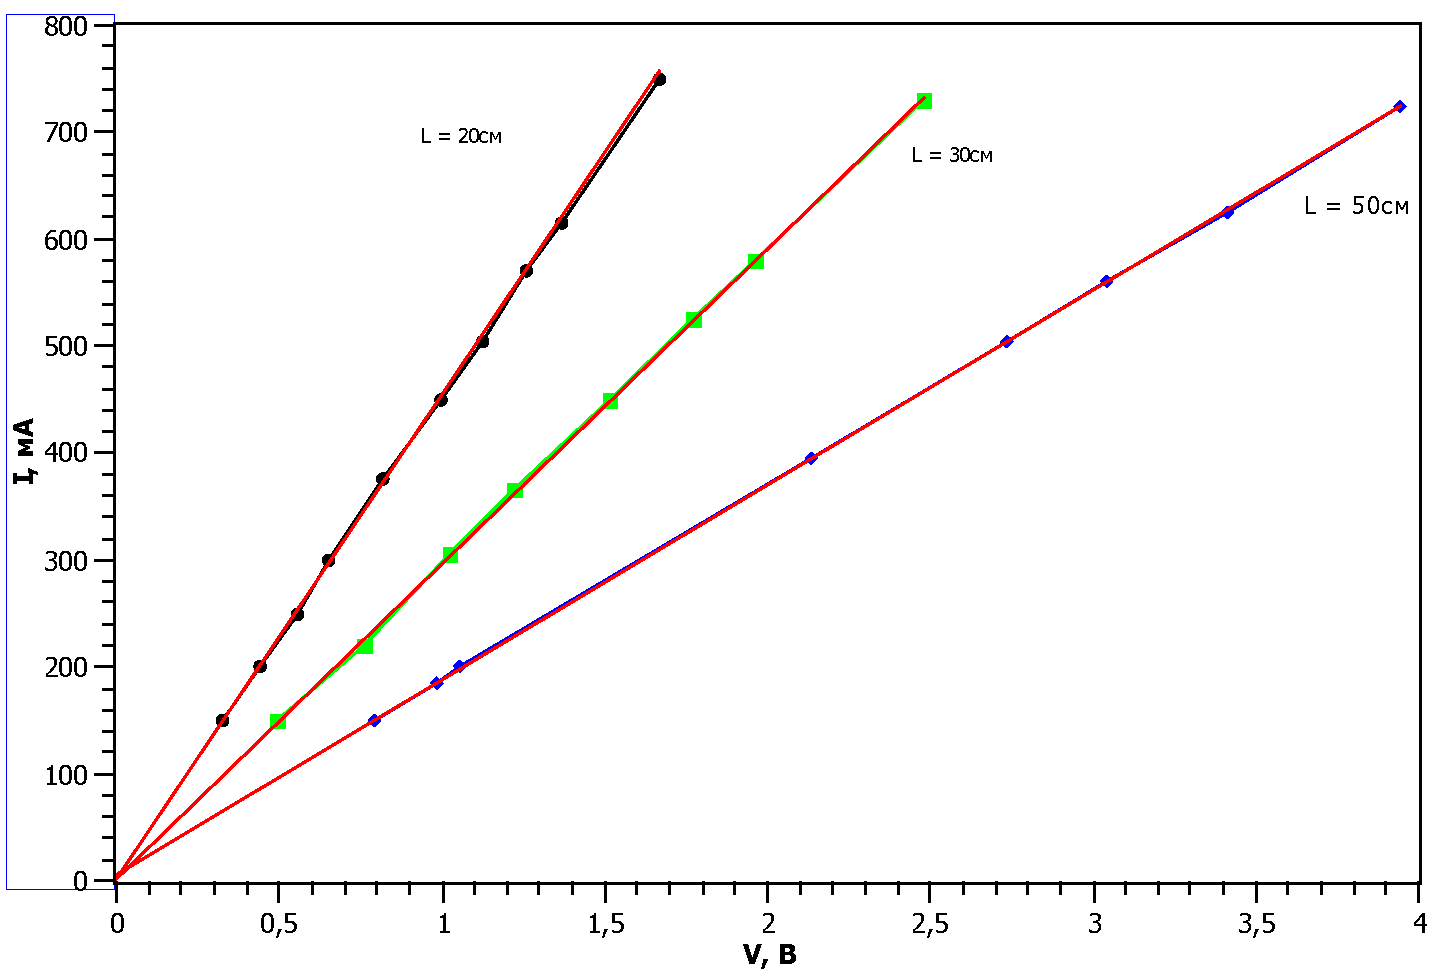
\includegraphics[width = 18cm]{graphics.pdf}}
		\caption{ВАХи}
		\label{fig:image}
	\end{figure}
	
	\newpage
	
	9. Для каждой длины $l$ находим среднее значение сопротивления по угловому коэффициенту соответствующей прямой: 
	$R_\text{ср} = V/I$, где $V$ и $I$ --- значения тока и напряжения, взятые на прямой в некоторой точке у ее конца.
	
	\vspace{0.5cm}
	10. Погрешность $R_\text{ср}$ оценим по формуле
	
	$$\frac{\sigma_{R_\text{ср}}}{R_\text{ср}} = \sqrt{\left(\frac{\sigma_V}{V}\right)^2 + \left(\frac{\sigma_I}{I}\right)^2}$$

	где $I$ и $V$ --- максимальные значения силы тока и напряжения, полученные в эксперименте, а $\sigma_I$ и $\sigma_V$ - 
	среднеквадратичные ошибки измерения вольтметром и амперметром.
	
	Ошибка $\sigma_V = 0.001$ В (вольтметр электронный, при измерениях колебался четвертый знак после запятой).
	
	Ошибка $\sigma_I = x_n/2 = 3$ мА ($1/2$ цены деления).
	
	\vspace{0.5cm}
	11. Для всех трех длин $l$ вносим поправку в измеренное значение сопротивления по формуле:
	
	$$R_\text{n} = R_\text{ср} + \frac{R_\text{ср}^2}{R_V}$$
	
	В виду малости поправки считаем $\sigma_{R_\text{n}} = \sigma_{R_\text{ср}}$. Также так как $R_V \flqq R_\text{ср}$, то
	значения $R_\text{n}$ и $R_\text{ср}$ разлличаться практически не будут.
	
	\vspace{0.5cm}
	\begin{center}
	\begin{tabular}{|c|c|c|}
	\hline
	$ l_1 = 20$ см						& $l_2 = 30$ см 					& $l_3 = 50$ см\\
	\hline
	$R_\text{ср} = 2.223$ Ом			& $R_\text{ср} = 3.394$ Ом			& $R_\text{ср} = 5.441$ Ом\\
	\hline
	$R_\text{n} = 2.223$ Ом				& $R_\text{n} = 3.394$ Ом			& $R_\text{n} = 5.441$ Ом\\
	\hline
	$\sigma_{R_\text{n}} = 0.004$ Ом	& $\sigma_{R_\text{n}} = 0.004$ Ом	& $\sigma_{R_\text{n}} = 0.004$ Ом\\
	\hline
										& $R_0 = 3.407$ Ом					& $R_0 = 5.449$ Ом\\
	\hline
	\end{tabular}
	\end{center}

	
	\vspace{0.5cm}
	12. Заметим, что результаты измерений при помощи вольтметра и амперметра совпадают с результатами, полученными при помощи
	моста в пределах погрешности.
	
	\vspace{0.5cm}
	13. Определим удельное сопротивление нихрома $\rho$ и погрешность $\sigma_\rho$:
	
	$$\rho = \frac{R_\text{n}}{l}\frac{\pi d^2}{4}$$
	
	$$\frac{\sigma_\rho}{\rho} = \sqrt{\left(\frac{\sigma_R}{R}\right)^2 + \left(2\frac{\sigma_d}{d}\right) + 
	\left(\frac{\sigma_l}{l}\right)}$$	
	
	\vspace{0.5cm}
	\begin{center}
	\begin{tabular}{|c|c|c|}
	\hline
	$l,$ см 	& $\rho, 10^{-4}$ Ом*см 	& $\sigma_\rho, 10^{-6}$ Ом*см\\
	\hline
	20			& 1.13 						& 0.07\\
	\hline
	30			& 1.15						& 0.07\\
	\hline
	50			& 1.11						& 0.07\\ 
	\hline
	\end{tabular}
	\end{center}
	
	\vspace{1cm}
	Отсюда:	
	$$\boxed{\boxed{\rho = (1.13 \pm 0.07)*10^{-4}~\text{Ом*см}}}$$
	
	\vspace{1cm}
	Таким образом, мы определили удельное сопротивление нихромовой проволоки. 
	
	\newpage
	Список использованной литературы:
	
	\vspace{0.5cm}
	1. "Лабораторный практикум по общей физике: Учебное пособие. В трех томах. Т1. Механика"/А.Д.Гладун, Д.А.Александров,
	Ф.Ф.Игошин и др.; Под редакцией А.Д.Гладуна. --- МФТИ, 2004.
	
	2. "Набор и верстка в системе \LaTeX "/С.М.Львовский. --- 2003.
	
\end{document}
